\documentclass[a4paper,12pt]{article}

\usepackage[danish]{babel}
\usepackage[utf8]{inputenc}
\usepackage[pdftex]{graphicx}
\usepackage{subfigure}
\usepackage{usecases}
\usepackage{setspace}
\onehalfspacing
\usepackage{upquote}
\usepackage{color}
\definecolor{listinggray}{gray}{0.9}
\usepackage{listings}
\lstset{
	language=,
	literate=
		{æ}{{\ae}}1
		{ø}{{\o}}1
		{å}{{\aa}}1
		{Æ}{{\AE}}1
		{Ø}{{\O}}1
		{Å}{{\AA}}1,
	backgroundcolor=\color{listinggray},
	tabsize=3,
	rulecolor=,
	basicstyle=\scriptsize,
	aboveskip={1.5\baselineskip},
	columns=fixed,
	showstringspaces=false,
	extendedchars=true,
	breaklines=true,
	prebreak =\raisebox{0ex}[0ex][0ex]{\ensuremath{\hookleftarrow}},
	frame=single,
	showtabs=false,
	showspaces=false,
	showstringspaces=false,
	identifierstyle=\ttfamily,
	keywordstyle=\color[rgb]{0,0,1},
	commentstyle=\color[rgb]{0.133,0.545,0.133},
	stringstyle=\color[rgb]{0.627,0.126,0.941},
}
\usepackage[center,font=small,labelfont=bf,textfont=it]{caption}
\usepackage{enumerate}
\usepackage[numbers]{natbib}
\usepackage{hyperref}
\hypersetup{
	pdfborder = {0 0 0},
    colorlinks,
    citecolor=blue,
    filecolor=blue,
    linkcolor=blue,
    urlcolor=blue
}
\usepackage{parskip}
\setlength{\parindent}{15pt}

\begin{document}

\begin{titlepage}


\newcommand{\HRule}{\rule{\linewidth}{0.5mm}} % Defines a new command for the horizontal lines, change thickness here

\center % Center everything on the page

\textsc{\LARGE Københavns Universitet}\\[1.5cm] % Name of your university/college
\textsc{\Large Projektkursus Systemudvikling 2014}\\[0.5cm] % Major heading such as course name

\HRule \\[0.4cm]
{  \bfseries \large Open Source Bannerreklamesystem \\ \huge EasyAd}\\[0.4cm] % Title of your document
\HRule \\[1.5cm]

\begin{minipage}[t]{0.4\textwidth}
\begin{flushleft} \large
\emph{Projektgruppe:}


Signar Nielsen % Your name
\\
060585
\newline
\\
Aslak Niclasen
\\
060693
\end{flushleft}
\end{minipage}
~
\begin{minipage}[t]{0.4\textwidth}
\begin{flushright} \large
\emph{Instruktor:} \\
Aske Mottelson Clausen % Supervisor's Name
\end{flushright}
\end{minipage}\\[4cm]

{\large 14. maj 2014}\\[3cm] % Date, change the \today to a set date if you want to be precise

\end{titlepage}

\tableofcontents %generate table of content


\clearpage %clears float-buffer - inserting those missing - and starts new page

\section{Abstract}

Projektet Easy Ad er et open source bannerreklamesystem. Formålet med Easy Ad er at udvikle et systemet der er nemt og gratis at bruge. Systemet skal kunne downloades af mindre ikke-kommercielle foreninger og interesseorganisationer, der hverken har de fornødne midler til at købe dyre systemer eller den tekniske viden til at vedligeholde et sådan system.

Easy Ad skal udvikles til et firma ved navn Treu Media. Treu Media er specialiceret indenfor annoncesalg og en lang række andre medieudgivelser. Easy Ad skal gøre det nemt for Treu Media at administrere annoncer til deres mange kunder. Systemet skal derudover løse en lang række tekniske udfordringer, som f.eks. hvordan man sikrer med hvilken vægtning et banner bliver vist. Eller hvordan man undgår at samme banner bliver vist flere gang på samme hjemmeside.

Simon Shine er den tekniske kontaktperson og det er ham der sætter de tekniske krav til systemet. Jan Treu-Nielsen, Treu Media's ejer, vil være kontaktperson ved aftesting og opsætning af systemet. Projektet vil løbe fra marts og indtil ultimo juni. Systemet er en prototype og vil muligvis ikke være færdig udviklet ved projektets udgang. 

\newpage

\section{Indledning}

Ifølge en rapport fra Danske Medier Research\footnote{\url{ http://www.fdim.dk/sites/default/files/mediearkiv/rapporter/danskernes\_brug\_af\_internettet\_2012\_rapport.pdf}} om danskernes internetforbrug er adgang til internettet fra hjemmet steget fra 83\% til 92\% på blot 4 år - fra 2007 til 2011. I takt med den stigende grad af internetforbrug anvender annoncører de digitale medier til at ramme deres målgruppe.

Flere og flere virksomheder, interesseorganisationer og foreninger bliver derfor synlige på internettet med en hjemmeside eller profil på de sociale medier. De står alle overfor samme udfordring, nemlig hvordan man tjener penge på nettet. Den mest udbredte forretningsmodel er salg af annoncer på nettet. Der er to udfordringer ved at annoncere på nettet; den ene er den tekniske udfordring ved at selv skulle vedligeholde et bannersystem, og den anden er den økonomiske udfordring ved at skulle købe sig adgang til et bannersystem eller den nødvendige tekniske viden. Vores system er et forsøg på at løse disse to problemer.

\section{IT-projektets formål og rammer}

Projektet har til formål at udvikle et open source bannerreklamesystem. Nedenfor ses projektets overordnede rammer og formål beskrevet i faktor-kriteriet. 

\subsection{FACTOR-kriteriet}

\large{\bf{F}}\normalsize{unctionality
\\
- Visning af bannere med forskellig vægtning
\newline
- Tidsbestemt/antalsbestemt bannervisning 
\newline
- Oprettelse af kunder 
\newline
- Oprettelse af grupper
\newline
- Oprettelse af bannere}
\newline
\newline
\large{\bf{A}}\normalsize{pplication domain
\\
- Medarbejdere tilknyttet Treu media}
\newline
\newline
\large{\bf{C}}\normalsize{onditions\\
- Skal kunne bruges på tværs af browsere\\
- Skjult for brugere af hjemmesider\\
- Open source}
\newline
\newline
\large{\bf{T}}\normalsize{echnology\\
- Web-teknologi: html, css, php, javascript.\\
- Databaser: MySQL\\
- Webserver: Apache}
\newline
\newline
\large{\bf{O}}\normalsize{bjects\\
- Bannere/Reklamer
\newline
- Administratorer
\newline
- Kunder
\newline
- Grupper}
\newline
\newline
\large{\bf{R}}\normalsize{esponsibility\\
- Holder styr på banner visning}

\section{Kravspecifikation for IT-løsningen}
\subsection{Funktionelle og ikke-funktionelle krav}
\textbf{Funktionelle krav}
\\
Funktionelle krav beskriver interaktionen mellem brugeren og systemet - uden at systemet fysisk, eller i praksis, er implementeret. Funktionelle krav siger noget om, hvordan systemet skal fungere, forventet input til systemet og forventet output fra systemet. De praktiske, eller fysiske, krav til systemet er beskrevet i ikke-funktionelle krav nedenunder.

EasyAd er et system, som gør det muligt at vedligeholde reklamer på ens hjemmeside. Systemet er opbygget sådan, at det kan være ejeren af en hjemmeside der administrerer systemet, eller det er en tredje part, der administrerer systemet. I vores tilfælde er det Treu Media, der administrerer reklamer på andres hjemmesider. Man altid skal kunne logge på for at få adgang til systemet og for at kunne administrere reklamerne. Når man er logget på systemet, skal man oprette en hjemmeside, hvor reklamen skal vises, og derefter skal man oprette en zone, som reklamen hører til. Dette kan f.eks. være specielle steder på hjemmesider. Til sidst skal man oprette selve reklamen og tilføje den til en zone.

Hjemmesiden, der oprettes får et automatisk genereret "access token", som er dens kodeord. Det er et krav, at hjemmesiden skal sende et access token med i sit request til systemet. Vi bruger access token - og andre mekanismer - til at identificere hjemmesiden, både for at undgå misbrug, men også for at kunne hente de rigtige reklamer.

Zonerne bestemmer, hvor på siden, reklamen skal vises. Hvis man f.eks. kun ønsker at få en reklame vist på en underside, kan man lave en zone til undersiderne, mens man har en anden zone til forsiden.
\\
\\
\textbf{Ikke-funktionelle krav}
\\
Ikke-funktionelle krav er direkte krav til systemet, hvor og hvordan det skal fungere. Ikke-funktionelle krav bliver også kaldt kvalitets krav, det vil sige krav til kvaliteten af det system, eller program, man udvikler. Man kan f.eks. stille krav til performance, pris, sikkerhed og mange andre ting. 

Da ikke-funktionelle krav er et vidt begreb, har vi valgt at bruge FURPS+ modellen, som bogen også bruger. FURPS står for Functionality, Usability, Reliability, Performance and Supportability. Plusset står for under-kategorier, som også bliver kaldt constraints.

Her er de ikke-funktionelle krav:
\begin{itemize}
	\item \textbf{Functionality:} Systemet skal kunne håndtere (oprette, ændre og vise) reklamer på en hjemmeside. Dette kræver selvfølgelig, at alle involverede parter har adgang til internettet. Det vil sige, systemet, hjemmesiden og brugeren af hjemmesiden.
	\item \textbf{Usability:} Formålet med systemet er, at det skal være nemt at bruge for alle involverede parter. Både administratorer, hjemmesider og brugere. Da det er meget svært at definere, hvad er "nemt" at bruge, laver vi nogle user-tests, for at sikre os, at det faktisk er nemt at bruge. Da tiden og resourcerne er begrænsede, vil vi ikke teste, om systemet er nemt at sætte op. Vi er nødt til at prioritere, og derfor vil vi i stedet teste, om systemet er nemt at bruge, efter det er blevet sat op. Dette vil vi teste sammen med Treu Media, hvor vi vil lave et tænk-højt eksperiment. Det er også vigtigt, at systemetet fungerer på alle moderne browsere (IE8+, Safari, Chrome og Firefox). Dette kan nemt testes i f.eks. browserstack.com - hvis der er tid til det, vil vi udføre sådan en test.
	\item \textbf{Reliability:} Denne del er lidt udenfor vores kontrol, da vi ikke kan styre, hvor og i hvilket miljø systemet vil blive sat op. Der skal ikke være nogen software-forhindring for, at systemet skal kunne være tilgængeligt 24 timer i døgnet 365 dage om året. Hvis vi antager, at serveren altid har forbindelse til internettet, så sætter dette først og fremmest krav til serveren, både hardware og software. Serveren skal være dimensioneret til at kunne håndtere trafikken og softwaren skal være designet på en hensigtsmæssig måde, så den ikke bruger unødvendige resourcer.
	\item \textbf{Performance:} Det er et krav til systemet, at svartiden er så lav som overhoved muligt. Der er flere faktorer, der spiller ind, men først og fremmest er det internetforbindelsen, serveren og selve softwaren. Brugen skal ikke bemærke, at han venter på, at reklamerne loader. Dette kan gøres på forskellige måder, f.eks. ved at loade reklamerne asynkront ved hjælp af XHR-objektet i JavaScript, så siden bliver mere brugervenlig.
	\item \textbf{Supportability:} Systemet kan understøttes af enhver, da det er open-source. Systemet bliver udviklet i PHP, hvilket også er et open-source sprog.
\end{itemize}

\textbf{Constraints:} Systemet er webbaseret og vil blive udviklet i PHP. Derudover benytter vi andre webteknologier, som f.eks. HTML, CSS, JavaScript (jQuery). Projektet er open-source, men hvis man vil udvikle, eller udvide, systemet, kan man gøre det i PHP. Vi har valgt at benytte en MySQL-database. I forhold til reklamerne skal man kunne uploade almindelige billeder, videosekvenser og flash-filer. Vi har ikke taget en endelig stilling til, hvilke filtyper man skal have lov til at uploade.

\subsection{Højniveau use case model}
Vi har lavet et højniveau use case diagram, som viser aktørerne og systemets funktionalitet. Treu Media har mulighed for at administrere sites, zones, reklamer og har adgang til statistik for viste reklamer. Den besøgende får vist en reklame på den besøgte hjemmeside.

\centerline{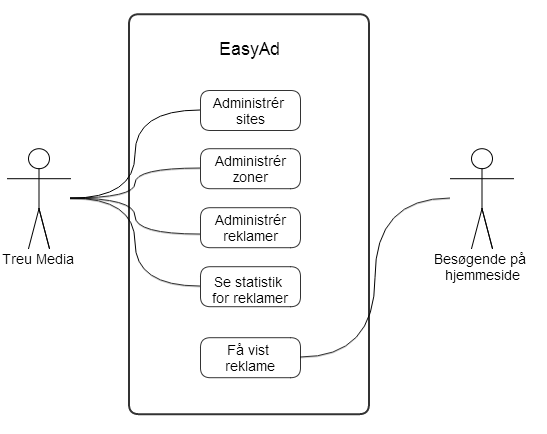
\includegraphics[scale=0.5]{hojniveau_diagram}}

\subsection{Tre use case modeller}
Da vores system frit kan installeres og bruges af alle, er der flere muligheder for opsætning, og der kan være flere aktører. I vores tilfælde har vi en interessent, som er Treu Media. Treu Media sælger reklamer for hjemmesider (som f.eks. www.ulandsnyt.dk), og vores use case model går ud på, at Treu Media skal oprette en reklame i systemet til hjemmesiden.

For at oprette en reklame i systemet, skal man først have oprettet en hjemmeside, hvor reklamen skal vises og derefter skal man oprette en zone på hjemmesiden, hvor reklamen hører til.

\centerline{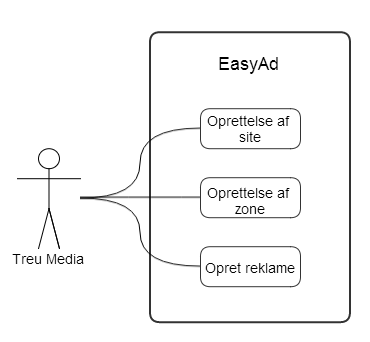
\includegraphics[scale=0.5]{treusecases}}

Vi starter med den første use case, hvor Treu Media skal oprette et site:

\begin{usecase}
\addtitle{Use case navn:}{Opret site}
\addfield{Aktør:}{Treu Media}
\addscenario{Flow:} {
	\item Tryk på "Customers"
	\item Tryk på "Create customer"
	\item Udfyld felterne "Name" og "URL". Begge felter skal udfyldes.
	\item Tryk på "Create customer now"
}
\addfield{Startbetingelser:}{Treu Media skal være logget på systemet}
\addfield{Slutresultat:}{En hjemmeside er oprettet i systemet}
\end{usecase}

Derefter tager vi en use case, hvor Treu Media skal oprette en zone, som tilhører et site:
\begin{usecase}
\addtitle{Use case navn:}{Opret zone}
\addfield{Aktør:}{Treu Media}
\addscenario{Flow:} {
	\item Opret en zone. Se tidligere use case
	\item Tryk på "Zones"
	\item Tryk på "Create zone"
	\item Udfyld feltet "Zone description" og vælg et site fra select-boksen
	\item Tryk på "Create zone now"
}
\addfield{Startbetingelser:}{Treu Media skal være logget på systemet. Der skal være oprettet et site}
\addfield{Slutresultat:}{En zone er oprettet i systemet}
\end{usecase}

Til sidst tager vi en use case, hvor Treu Media skal oprette en reklame, der tilhører en zone.
\begin{usecase}
\addtitle{Use case navn:}{Opret reklame}
\addfield{Aktør:}{Treu Media}
\addscenario{Flow:} {
	\item Opret et site. Se tidligere use case
	\item Opret en zone. Se tidligere use case
	\item Tryk på "Ads"
	\item Tryk på "Create ad"
	\item Felterne "Ad name", "Site name" og "Zone name" er påkrævede. De andre felter er valgfrie.
	\item Vælg reklamen fra din computer ved at trykke på "Vælg fil"
	\item Tryk på "Create ad now"
}
\addfield{Startbetingelser:}{Treu Media skal være logget på systemet. Der skal være oprettet et site og en tilhørende zone}
\addfield{Slutresultat:}{En reklame er oprettet i systemet}
\end{usecase}

\subsection{Klassediagram}
Vores klasser er følgende: administrator, site, zone og reklame. Forholdet mellem klasserne er, at flere zoner kan tilhøre et site, men flere reklamer kan tilhøre én zone. Derved kan flere reklamer også tilhøre et site.

\begin{figure}[h!]
  \centering
    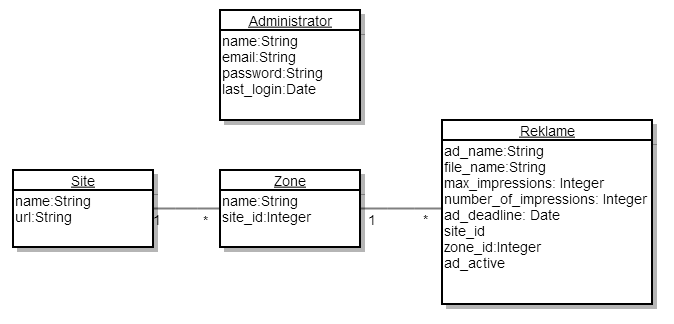
\includegraphics[scale=0.5]{klasse_diagram.png}
  \caption{Klassediagram}
\end{figure}

\subsection{Sekvensdiagram}
Sekvensdiagram over oprettelse af kunde.
\\
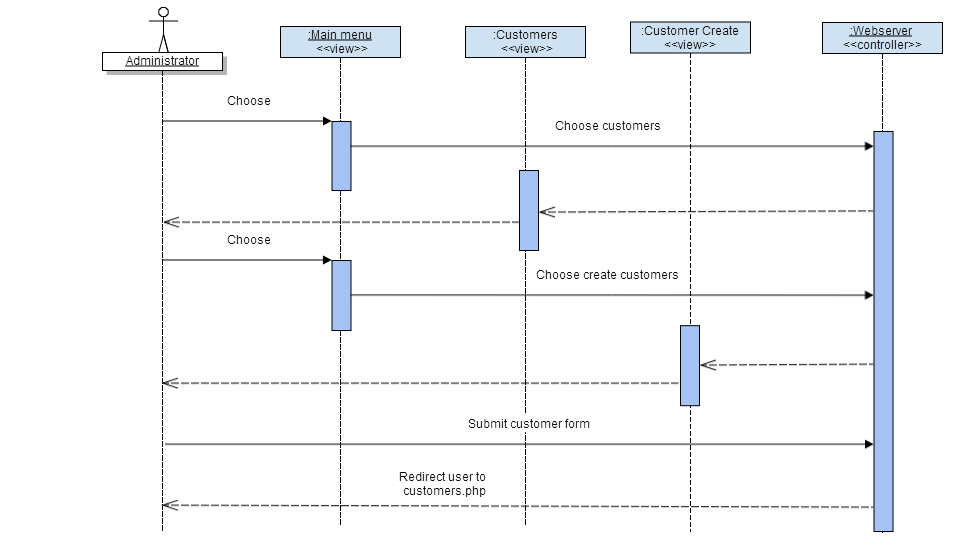
\includegraphics[width=\textwidth]{sekvensdiagram1.png}
\\
\\
Sekvensdiagram over oprettelse af gruppe
\\
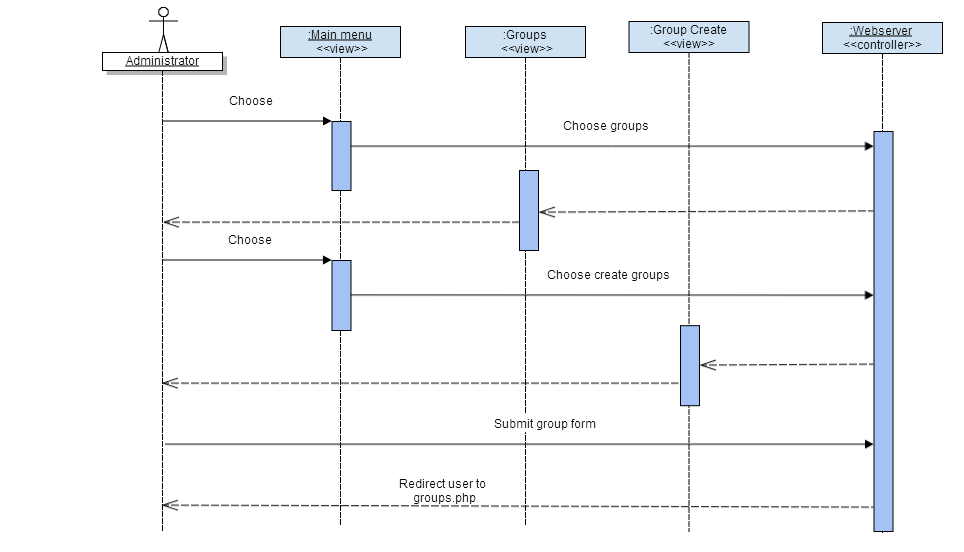
\includegraphics[width=\textwidth]{sekvensdiagram2.png}
\\
\\
Sekvensdiagram over oprettelse af reklame
\\
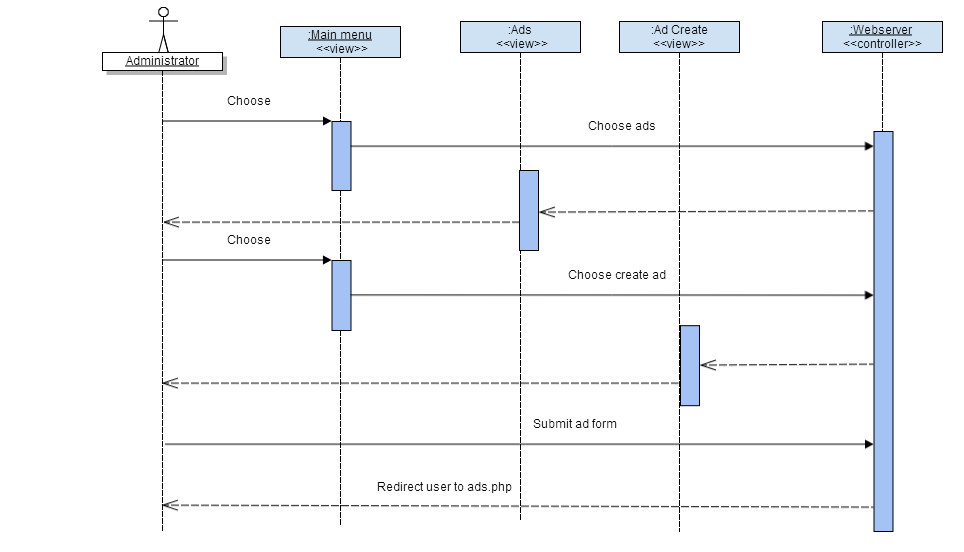
\includegraphics[width=\textwidth]{sekvensdiagram3.png}

\section{Systemdesign sammenfatning}
Fra delrapport 2 til delrapport 3 har vi valgt at ændre begreberne "customer" til "site" og "group" til "zoner", så vi undgår forvirring om, hvem er hvem og hvad er hvad. Det viser sig, at til hvert review, vi har fået, har der været tvivl omkring begreberne interessent, bruger og kunde. Nu er Treu Media interessenten og brugeren er en besøgende på en hjemmeside. Vi bruger ikke "kunde" længere.

Vi er nået dertil, at Treu Media kan oprette sites, zoner og reklamer. Vi har lavet en grov skitse af systemet, men mangler at implementere nogle funktioner, som f.eks. at give Treu Media mulighed for at ændre et site, zone og reklame. Vi skal også sørge for at beskytte imod SQL-injections og sikre os, at de krævede felter faktisk bliver udfyldt, når Treu Media f.eks. opretter en reklame. 

Den vigtigste funktion vi mangler, er at vise en reklame på en hjemmeside. Der findes flere muligheder for, hvordan vi kan lave denne del af systemet. Vi har diskuteret fordele og ulemper ved de forskellige muligheder, og har ikke truffet en endelig beslutning. Højst sandsynligt vælger vi en løsning, hvor kunden skal tilføje en javascript-fil til hjemmesiden, som henter og placerer reklamerne på hjemmesiden.

Vi mangler også at udføre et tænk-højt eksperiment, unit tests og at teste, at vores reklamer bliver vist det rigtige sted og at statistikken er rigtig. Dette vil vi meget gerne have udført til næste delrapport.

\section{Program- og systemtest}
Projektgruppen ønsker at teste systemet i flere omfang. Vi har planlagt at udføre et tænk-højt forsøg sammen med Treu Media og, hvis der er tid til det, et tænk-højt forsøg sammen med Simon Shine, som er teknisk kontakt. Formålet med tænk-højt forsøget er at teste vores brugergrænseflade.

Derudover vil vi lave unit tests og teste, at systemet registrerer visning af reklamer rigtigt. Beskrivelse følger..

\subsection{Interne test}
Ved de interne test skal vi benytte os af unit testing. Denne testing skal finde sit ståsted i matematikken, og vil omhandle en form for tællemekanisme. Gruppen ønsker længere fremme i projektet at teste antallet af visninger af reklamer på hjemmesider. Vi skal altså forsøge at skabe en reklamevisning internt i programmet et kendt antal gange. Vores tællemekanisme skal således beregne et resultat udfra vores reklamers visning. Dette resultat skal herefter sammenlignes med det forventede antal visninger fra start.

En konkret måde at løse gruppens problem her, kunne være på følgende måde: uploade en reklame, sende fiktive requests til en hjemmeside med dette banner. Herved kunne gruppens tællemekanisme aflæse om requesten bliver behandlet korrekt og dermed registrere en visning. Dette ville resultere i, at man kan tælle antallet af requests som der er blevet behandlet i processen og gruppen ville hurtigt kunne se om det forventede resultat stemte overens med det reelle resultat fra vores tællemekanisme.

\subsection{Eksterne test}
Projektgruppen regner desuden med testning af systemets nuværende brugergrænseflade. Gruppen vil lave et tænk-højt forsøg, som indebærer at interessenten benytter sig af systemet. Vi vil på forhånd stille nogle use cases (eller opgaver), som vi gerne vil have testet, og så sætter vi interessenten til at udføre disse uses cases. Formålet med forsøget er at teste brugervenligheden i vores brugergrænseflade. Vi vil gerne dokumentere testen ved at optage skærmbilledet og det, interessenten siger, mens han bruger systemet. Vi vil også være tilstede, mens testen udføres for at besvare eventuelle spørgsmål eller stille andre opgaver, hvis der er behov for det.


\section{Brugergrænseflade og interaktionsdesign}
Hvis man trykker på "Sites" kommer man ind på oversigten over sine hjemmesider. Hver hjemmeside får tildelt et "access token", som er dens password. Hjemmesiden skal indsætte sit access token på sin hjemmeside, sådan at vores system kan identificere hjemmesiden.
\\
\centerline{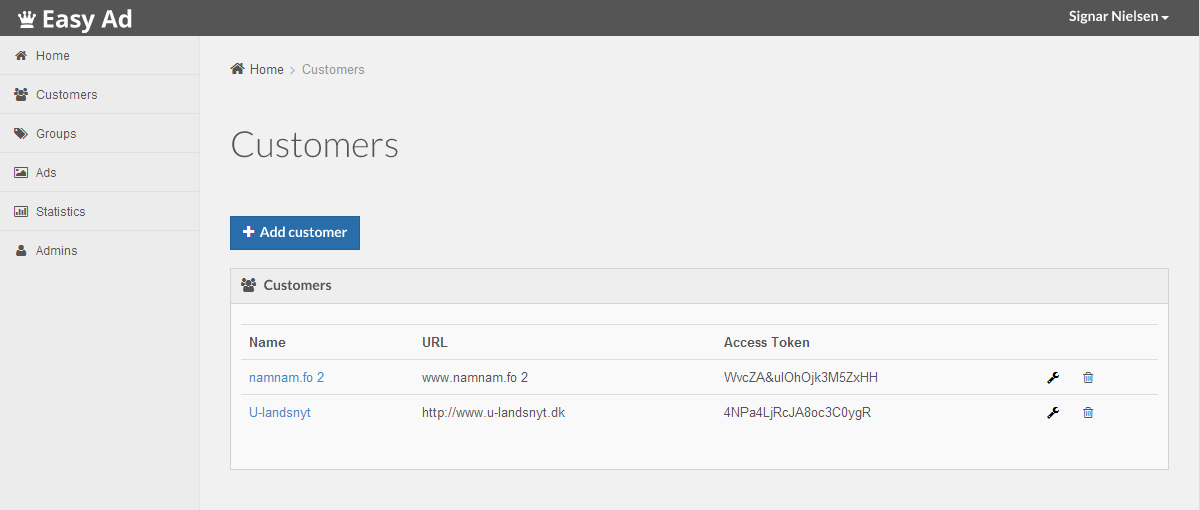
\includegraphics[width=\textwidth]{customers.png}}
\newline
\newline
\newline
Hvis man er inde på sites og trykker på "Create site" får man lov at tilføje en hjemmeside.
\\
\centerline{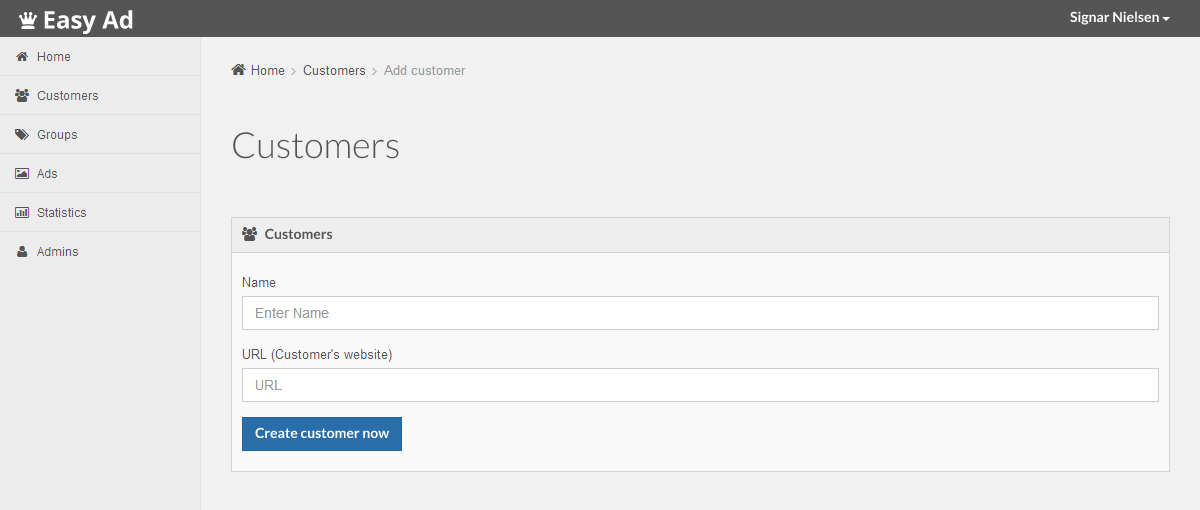
\includegraphics[width=\textwidth]{customer_add.png}}
\newline
\newline
\newline
Når man lige er logget ind, kan man trykke på "Ads" for at få en oversigt over alle reklamerne. I oversigten ser man også, hvilken zone og hvilken kunde, reklamen hører til.
\\
\centerline{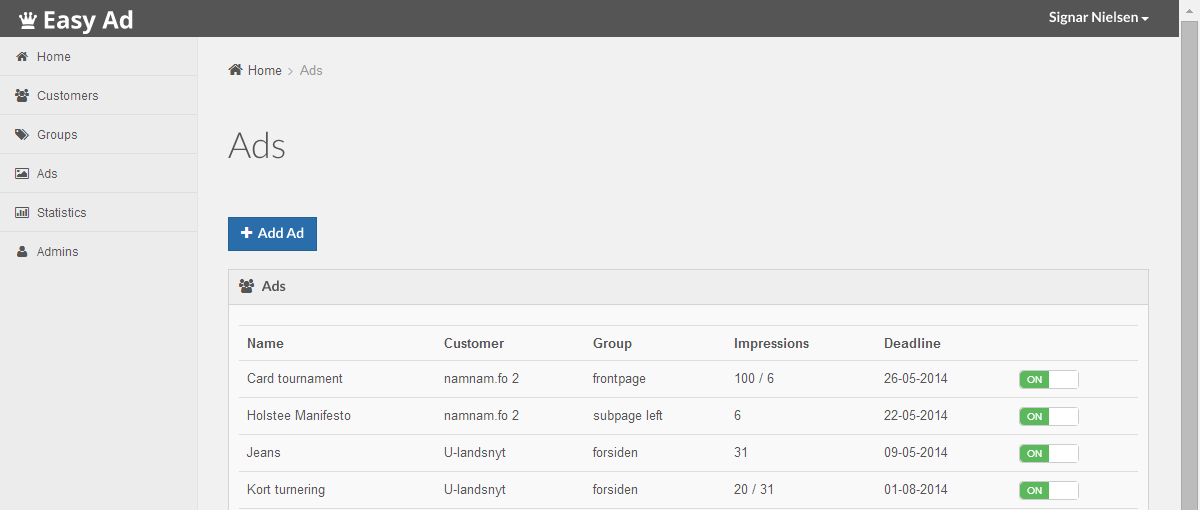
\includegraphics[width=\textwidth]{ads.png}}
\newline
\newline
\newline
Hvis man begærer at oprette en ny reklame skal man blot trykke på "Ads" og derefter "Create Ad". Derefter kommer man ind på siden, hvor man kan oprette en reklame. Der er tre felter, der er påkrævet, og det er "Ad name", "Site name" og "Zone name". Når man er færdig, trykker man blot på "Create ad now".
\\
\centerline{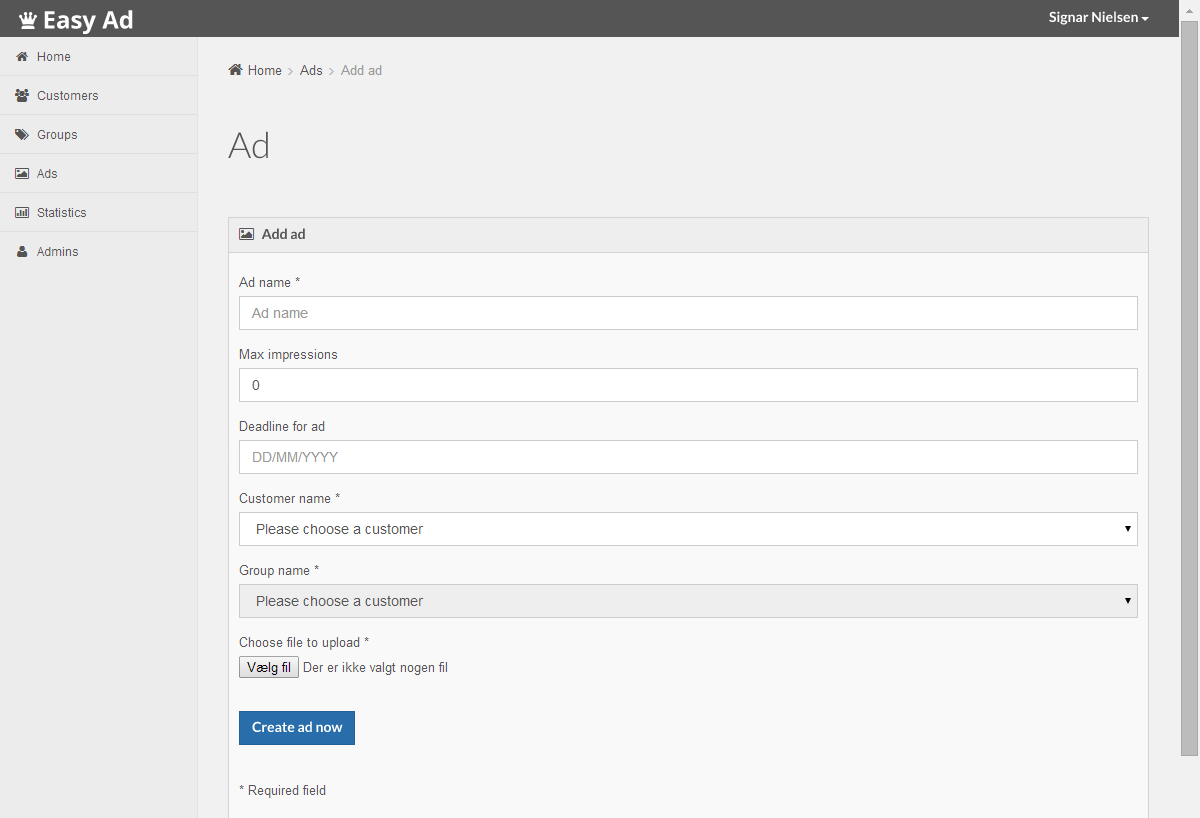
\includegraphics[width=\textwidth]{ad_add.png}}
\newline
\newline
\newline
Som administrator får man også en oversigt over statistik over viste reklamer.
\\
\centerline{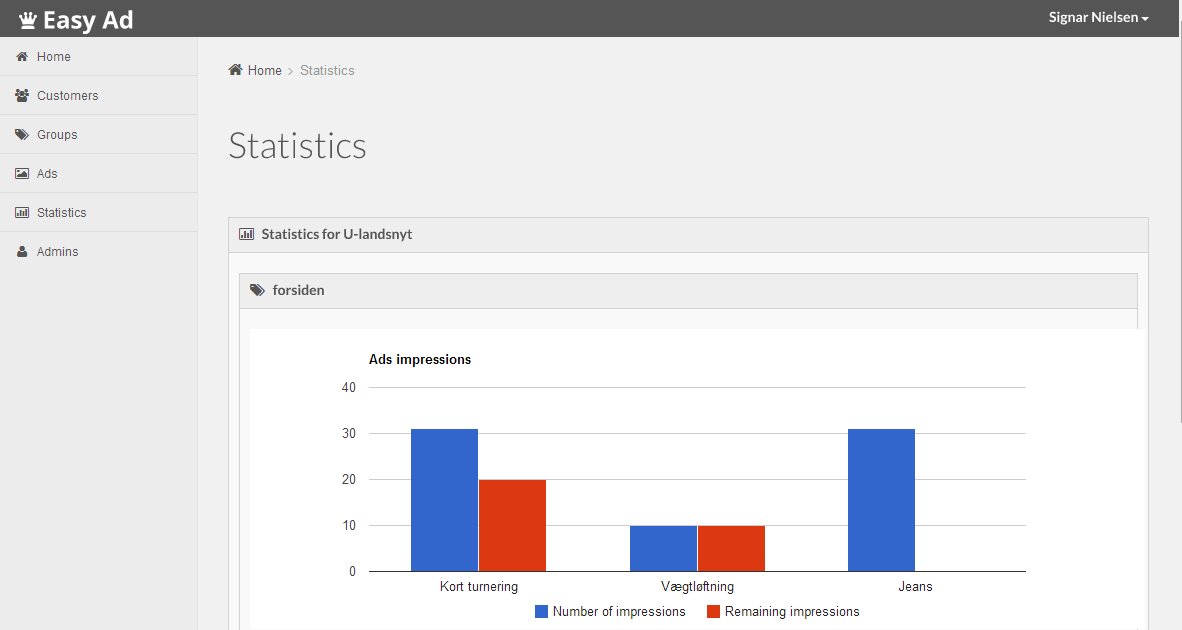
\includegraphics[width=\textwidth]{statistics.png}}

\subsection*{Audio visuel præsentation}
Vi har lavet en demonstration af vores brugergrænseflade, som vi har uploaded til youtube:
\newline
\url{http://bit.ly/1oLR4JC}

\subsection*{Tænke-højt forsøg}
Vi har ikke udført et tænke-højt forsøg endnu, men det har vi planer om at nå til næste rapport.


\section{Versionstyring}
Vi benytter GitHub til versionstyring. Vores projekt ligger på
\newline
\url{http://github.com/AslakNiclasen/ProjektOpgave}.
\newline
\\
Da vi commiter flere gange i løbet af en programmerings-session, giver det ikke rigtig nogen mening at vedhæfte vores commit-log fordi den er så lang. Den er også offentligt tilgængelig, så alle kan gå ind og se den. Vi har heller ikke valgt at vedhæfte vores kode, da den også er offentlig.
\newline
\\
Vi har valgt at commite tit, så vi undgår risikoen ved at en stor del af arbejdet går tabt, hvis uheldet er ude. Grunden til, at Aslak ikke har commited lige så ofte, som de andre er fordi, at han har problemer med Git på sin computer.

\section{Projektsamarbejdet}
\subsection{Hvad går godt?}
\textbf{Internt}
\newline
Projektgruppen har i løbet af de sidste par uger mødtes flere gange om ugen, og disse har været yderst produktive. Til disse forskellige møder har vi på dagen planlagt en dagsorden, og al opgaveskrivningen er foregået sammen på selve dagen. Arbejdet mellem gruppen internt fungerer meget gnidningsfrit og vi opfylder hindandens krav, og de krav der stilles til opgaven. Vi møder velforberedte og friske, således at dagenene hvor vi har valgt at mødes bliver så konstruktive som overhoved muligt. Det har fungeret fremragende og vi er nu på et stadie i projektet, hvor vi ikke skal programmere så meget mere, men hvor vi skal fokusere på rapporterne.
\\
\\
\textbf{Med interessent}
\\
Vi har ikke haft et møde med vores interessent til dags dato, men vi har haft to møder og mailkorrespondance til vores mellemled mellem os og interessenten. Interessenten giver klart udtryk for et frugtbart samarbejde, med mulighed for fremtidige møder efter vores ønske - det kommer vi selvfølgelig til at benytte os af. Vi er på nuværende tidpunkt klar til at teste programmet med interessenten og vi arbejder på at få skabt en god kontakt, således at testningen sker snarest og kan fremlægges i den kommende delrapport 4.
\\
\\
\subsection{Hvad går mindre godt?}
\textbf{Internt}
\\
Vi har valgt, at alle bidrag til github, sker udelukkende gennem et gruppemedlem, da vi så langt som vi er i vores projekt. Dette skyldes at github og visse udgaver af mac er meget komplicerede at få til at fungere sammen. Det har derfor ikke været muligt at optimere dette problem med en virtuel maskine. Samtidigt med at vi desværre har mistet et gruppemedlem, Amanda, har andre muligheder åbnet sig. Vi kan af den grund nemmere mødes. Dette har resulteret i ovenstående aftale omkring github, da begge medlemmer sidder sammen og overfører filer hurtigere, til hinanden, end hvis vi skulle benytte den virtuelle maskine på den ene computer.
Der er selvfølgelig mere arbejde i forhold til rapportskrivningen, da vi er nået langt i projektet på nuværende tidspunkt. Begge medlemmer er så fleksible at vi mødes op til 5 gange om ugen. Således når vi stadig at lave den mængde af arbejde rapportskrivningen kræver.
\\
\\
\textbf{Med interessent}
\\
I og med at gruppen ikke har haft møde med interessenten, er det svært at foretage en vurdering af dette punkt. Vi synes dog i og med at interessenten viser meget interesse og er nem at få kontakt til telefonisk, at vi ikke har nogen problematik her. Vi regner med at få kontakt til interessenten i næste uge, og aftale nærmere detaljer omkring testning af projektet.
\\
\\
\subsection{Hvilke optimeringer i forhold til projektarbejdet kan vi foretage?}
\textbf{Internt}
\\
Vi kan ikke optimere vores arbejde mere end vores nuværende indsats. Vores mødeplan kan ikke optimeres mere, da vi mødes så tit. Produktiviteten under disse møder kan heller ikke optimeres yderligere. Begge gruppemedlemmer yder en meget stor indsats og projektet fortsætter stadigt fast fremad.
\\
\\
\textbf{Med interessent}
\\
Som nævnt, tager vi snarest kontakt til interessenten, og det betyder, at vi ikke kan gøre mere end at aftale mødetidspunkt og herefter beslutte fremtidige dagsordner med interessenten, hvis dette kræves.

\section{Reviews}
\subsection{Review: No Silver Bullet}
Forfatteren til artiklen beskriver det største problem indenfor Software Engineering. Han bruger en metafor, der skaber en omliggende ramme for problemet artiklen omfatter. Metaforen Silver Bullet referer til det middel, i gamle folkemyter, som en varulv kunne  bekæmpes med. Varulven repræsenterer noget der med det samme kan gå fra et stadie til et andet. Noget harmløst og kendt, til et monster uden kendte grænser \cite[side~181]{nsb}. Denne Silver Bullet er således et desperat kald fra software verdenen om at nedlægge problemet ved Software Engineering, nemlig hvordan en udviklingsproces i form af softwaren, hvad enten det er nye begreber, mennesker eller fysiske projekter, kan optimeres. 

Artiklen tager sit standpunkt i fire hovedområder som forfatteren mener kan mindske problematikken. Disse fire punkter knytter sig til den essentielle del af software Engineering og ikke den acidentale. Forskellen på disse er at finde i en konceptuel mening. Den essentielle del af software Engineering som problemet er at finde i, skal forstås som de problematikker der ligger begravet i hele naturen af Software. Den acidentale del af softwaren betegner de problematikker som opstår gennem produktionen af software, men ikke tilhører den bagvedliggende natur \cite[side~182]{nsb}.
\newline
\newline
De fire punkter  der nævnes er:
\newline
Udnyttelse af hele software markedets ressourcer.
\newline
Brugen af prototyper som en del af iterations-design for at skabe software krav.
\newline
Konceptet med at software gror og udfolder sig organisk
\newline
Opdage og udvikle de fremragende konceptuelle designer i kommende generationer.
\cite[side~180]{nsb}

Igennem artiklen beskrives den essentielle del, og den acidentale del mere udførligt. De fire punkter bruges som argumenter igennem artiklen og opsættes således at man kan se hvordan de skal løse problemet. 
Vi ikke har en Silver Bullet på nuværende tidspunkt, (vi får næppe en heller) men benytter vi punkterne kan vi komme tættere på målet. ”There is no royal road, but there is a road” \cite[side~181]{nsb}.

Artiklen er meget spændende, da den opstiller et hidtil uopklaret problem. Men problemet viser sig at være det mest interessante problem i vores historie indenfor Software udvikling. Andre kildeartikler som f.eks. a rational design process: why and how to fake it og Designing for Usability: Key Principles and What Designers Think, har i et mindre omfang også beskæftiget sig med dette problem. Men de fraviger fra den egentlige problemstilling som artiklen her beskæftiger sig med, og ser på den acidentale del af problem, fremfor den essentielle del.

Også bogen OOSE adresserer problemet implicit i hele dens omfang. Visse af bogens kapitler benytter sig af metodikker og teoretiske virkemidler til at hjælpe med den praktiske udvikling af at software system. Metodikkerne og teorien bag disse virkemidler er meget tæt knyttet til det essentielle Software Engineering problem som denne artikel adresserer. Et eksempel kunne være: recall punkt tre og fire, i samspil.  Det vælger vi at sætte op imod en agil arbejdsproces. Her vil både softwaren og menneskerne gro sideløbende som et projekt forløber. Alle ressourcer bliver udnyttet til fulde, og man gennemgår en cyklus – heraf er nu de to første punkter fra artiklen også blevet inddraget i projektforløbet. Alle dele implicit, men de fremmer softwareudviklingen frugtbart, fordi de alle er nødvendige.

Det samme oplever vi også praktisk i vores projekt. Hvordan en arbejdscyklus giver designeren mulighed for at udfolde sig selv, men også udfolde systemet løbende i processen. Det er ikke muligt konkret at sætte et projekt som vores i reel kontekst til problemet der adresseres i artiklen, da det er på et mere overordnet plan. Som tidligere nævnt, har vi på nuværende tidspunkt ikke en silver bullet til rådighed, men hvis vi udnytter alle vores ressourcer på en hensigtsmæssig måde, vil projektet også blive mest frugtbart.   

\subsection{Review: Mocking-it-up or Hands-on The Future}
Artiklen som danskeren, Morten Kyng og svenskeren, Pelle Ehn, har skrevet omhandler det, som de kalder "participatory design". Artiklen er skrevet i 1991 og den beskriver, hvordan man kan designe ting med modeller (mockups), uden virkelige prototyper af det designede ting. De arbejde begge med et projekt, som kaldes Utopia. Deres opgave er at designe en arbejdsproces, som tager udgangspunkt i journalistens og typografens arbejde i 70erne, hvor linjerne for hvem laver hvad, er ved at blive lidt slørede, og hvor spændingen mellem journalisterne og typograferne er ret høj. De beskriver, hvordan man hurtigt og biligt kan opsætte en model af en arbejdeproces, som i dette tilfælde blandt andet består af computere, printere og software, hvor brugeren er involveret, ved hjælp af kartong og andre billige materialer. Fordelen ved brug af modeller er, at man nemt kan lave ændringer i designet, uden at det koster ekstra tid eller penge. En anden stor fordel ved disse modeller er, at alle har evnerne til at ændre i dem, fordi det kræver ikke viden inden programmering eller industriel design. Den største fordel ved modeller, fremfor beskrivelser på papir, er at den lægger op til hands-on erfaring og det opmuntrer involvering af brugeren.

Artiklen leder tankerne til Scrum, som er en metode inden softwareudvikling. Scrum er en del af de agile metoder inden for software udvikling. Scrum går ud på, at man har et Scrum team, som består af scrum master, produktejer og udviklings teamet. Scrum master har ansvaret for at produktet bliver leveret i henhold til kravene til kunden og til den tiden. Produkt ejeren repræsenterer typisk dem, der skal bruge produktet når det er færdigt. Produkt ejeren er med i hele forløbet, mens produktet bliver udviklet, på samme måde som modellerne og den "participatory design"-proces lagde op til. Produkt ejeren kan godt komme med ændringer til produktet mens det bliver udviklet, hvis der er behov for det, og Scrum udviklingsteamet udfører de ønskede ændringer. På denne måde sker der en iteration af krav til systemet og udvikling af kravene, hvorfor også det er en agil metode.

Vi kender også fra arbejde inden for softwareudvikling, at man bruger modeller, før man går i gang med at udvikle produktet. Signar har været med til at udvikle software, hvor man bruger papir, blyant og en saks til at lave modeller af produktet. Han har også været med til at bruge andre værktøjer, som f.eks. software, til at tegne modeller af produktet. Det er helt klart en fordel at bruge papir og blyant, når man skal lave den første skitse, fordi det er ekstremt hurtigt at ændre og det koster ikke noget. Det har også sin fordel at bruge software-værktøjer til at lave modeller, som f.eks. Photoshop eller Moqups.com, fordi det er et skridt tættere på det virklige produkt.

\newpage
\section{Litteraturliste}

\begin{thebibliography}{9}

\bibitem{nsb}
	Brooks, F. P. (1986), 
	\emph{No silver bullet}, Proc. of the IFIP Tenth World Computing Conference, edited by H.-J. Kugler (1986), pp. 1069-76. Reprinted version from the book Brooks, F. P. (1995), The mythical manmonth: Essays on software engineering, Addison-Wesley Publishing.
	
\bibitem{miu}
	Ehn, P. and Kyng, M. (1991), \emph{Cardboard computers: Mocking-it-up or hands-on the future}. In Greenbaum, J. and Kyng, M., editors, (1991), in: Design at Work: Cooperative Design of Computer Systems, pages 169–195. Lawrence Erlbaum Associates.
\end{thebibliography}

\end{document}